
\section{Deliverable 5: Differences in Optimizers (Sinusoidal dataset)}


\begin{solve}    

\begin{figure}[H]
    \centering
    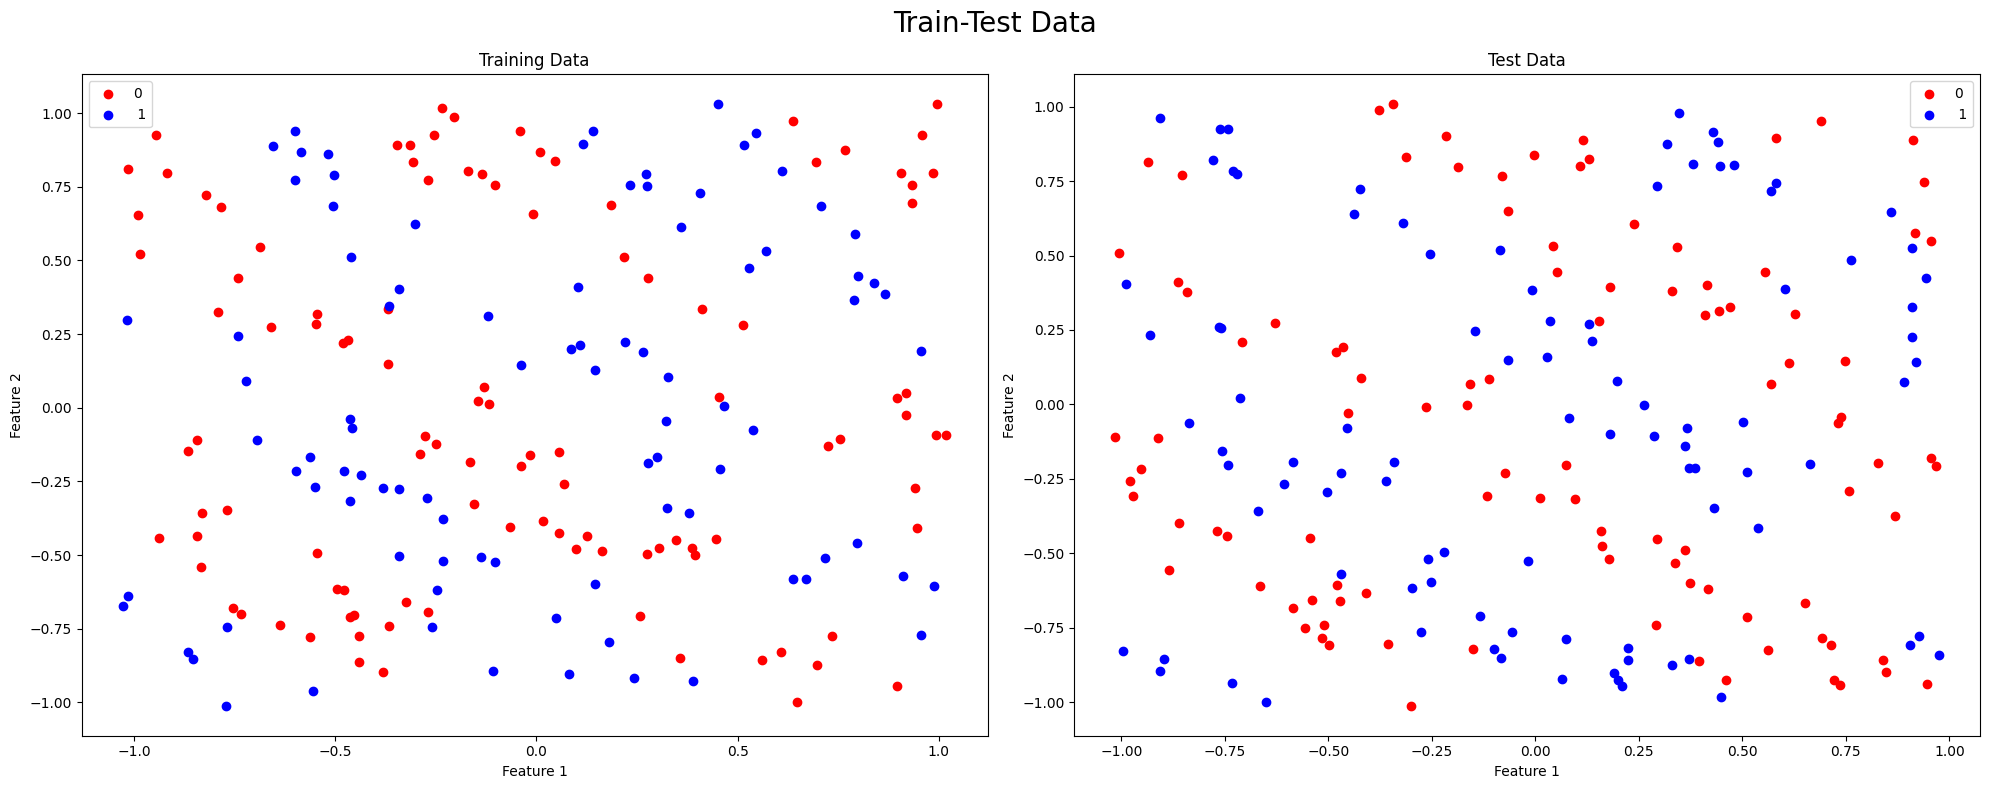
\includegraphics[width=0.7\textwidth]{plots/sinusoid_dataset.png}
    \caption{Sinusoidal dataset (train, test set with 200 points each)}
\end{figure}

\subsection*{Model Description}

\begin{lstlisting}[language=python]
dim_in, dim_out = x_train.shape[1], 2
hidden_neuron_list = [8, 16, 32, 8]
activation_list = ['ReLU','ReLU', 'ReLU','ReLU','LinearActivation'] 
# linear at the last layer because sigmoiding in the loss function forward pass for CrossEntropyLoss
opt_init = 'xavier'
opt_loss = CrossEntropyLoss()
mlp = MLP(dim_in, dim_out, hidden_neuron_list, activation_list, opt_init)
print(mlp.summary())
-----------------------------------------------------------------
Model Summary
-------------
Layer 1: Linear - A Dim: 2, Output Dim: 8, Parameters: 24
Layer 2: ReLU
Layer 3: Linear - A Dim: 8, Output Dim: 16, Parameters: 144
Layer 4: ReLU
Layer 5: Linear - A Dim: 16, Output Dim: 32, Parameters: 544
Layer 6: ReLU
Layer 7: Linear - A Dim: 32, Output Dim: 8, Parameters: 264
Layer 8: ReLU
Layer 9: Linear - A Dim: 8, Output Dim: 2, Parameters: 18
Layer 10: LinearActivation
Total Parameters: 994
    \end{lstlisting}


\subsection{Optimizer Performance}
We see that the Adam optimizer with learning rate 0.01 performs the best in terms of loss and accuracy. The decision boundary is also the most accurate. The performacne for the SGD optimizer with learning rate 0.01 and momentum is the second best (with lesser train accuracy but simlar test performance). We do see that tho the decision boundary is over fitting to train in this case.

Adam optimizer with learning rate 0.001 is lesser accurate, followed by vanilla SGD which gives the worst performance in terms of loss and accuracy. The decision boundary is also the most inaccurate.

\subsection{ \textcolor{red}{Best Performance: MLP with Adam Optimizer of learning rate 0.01 and default parameters} }

\begin{figure}[H]
    \centering
    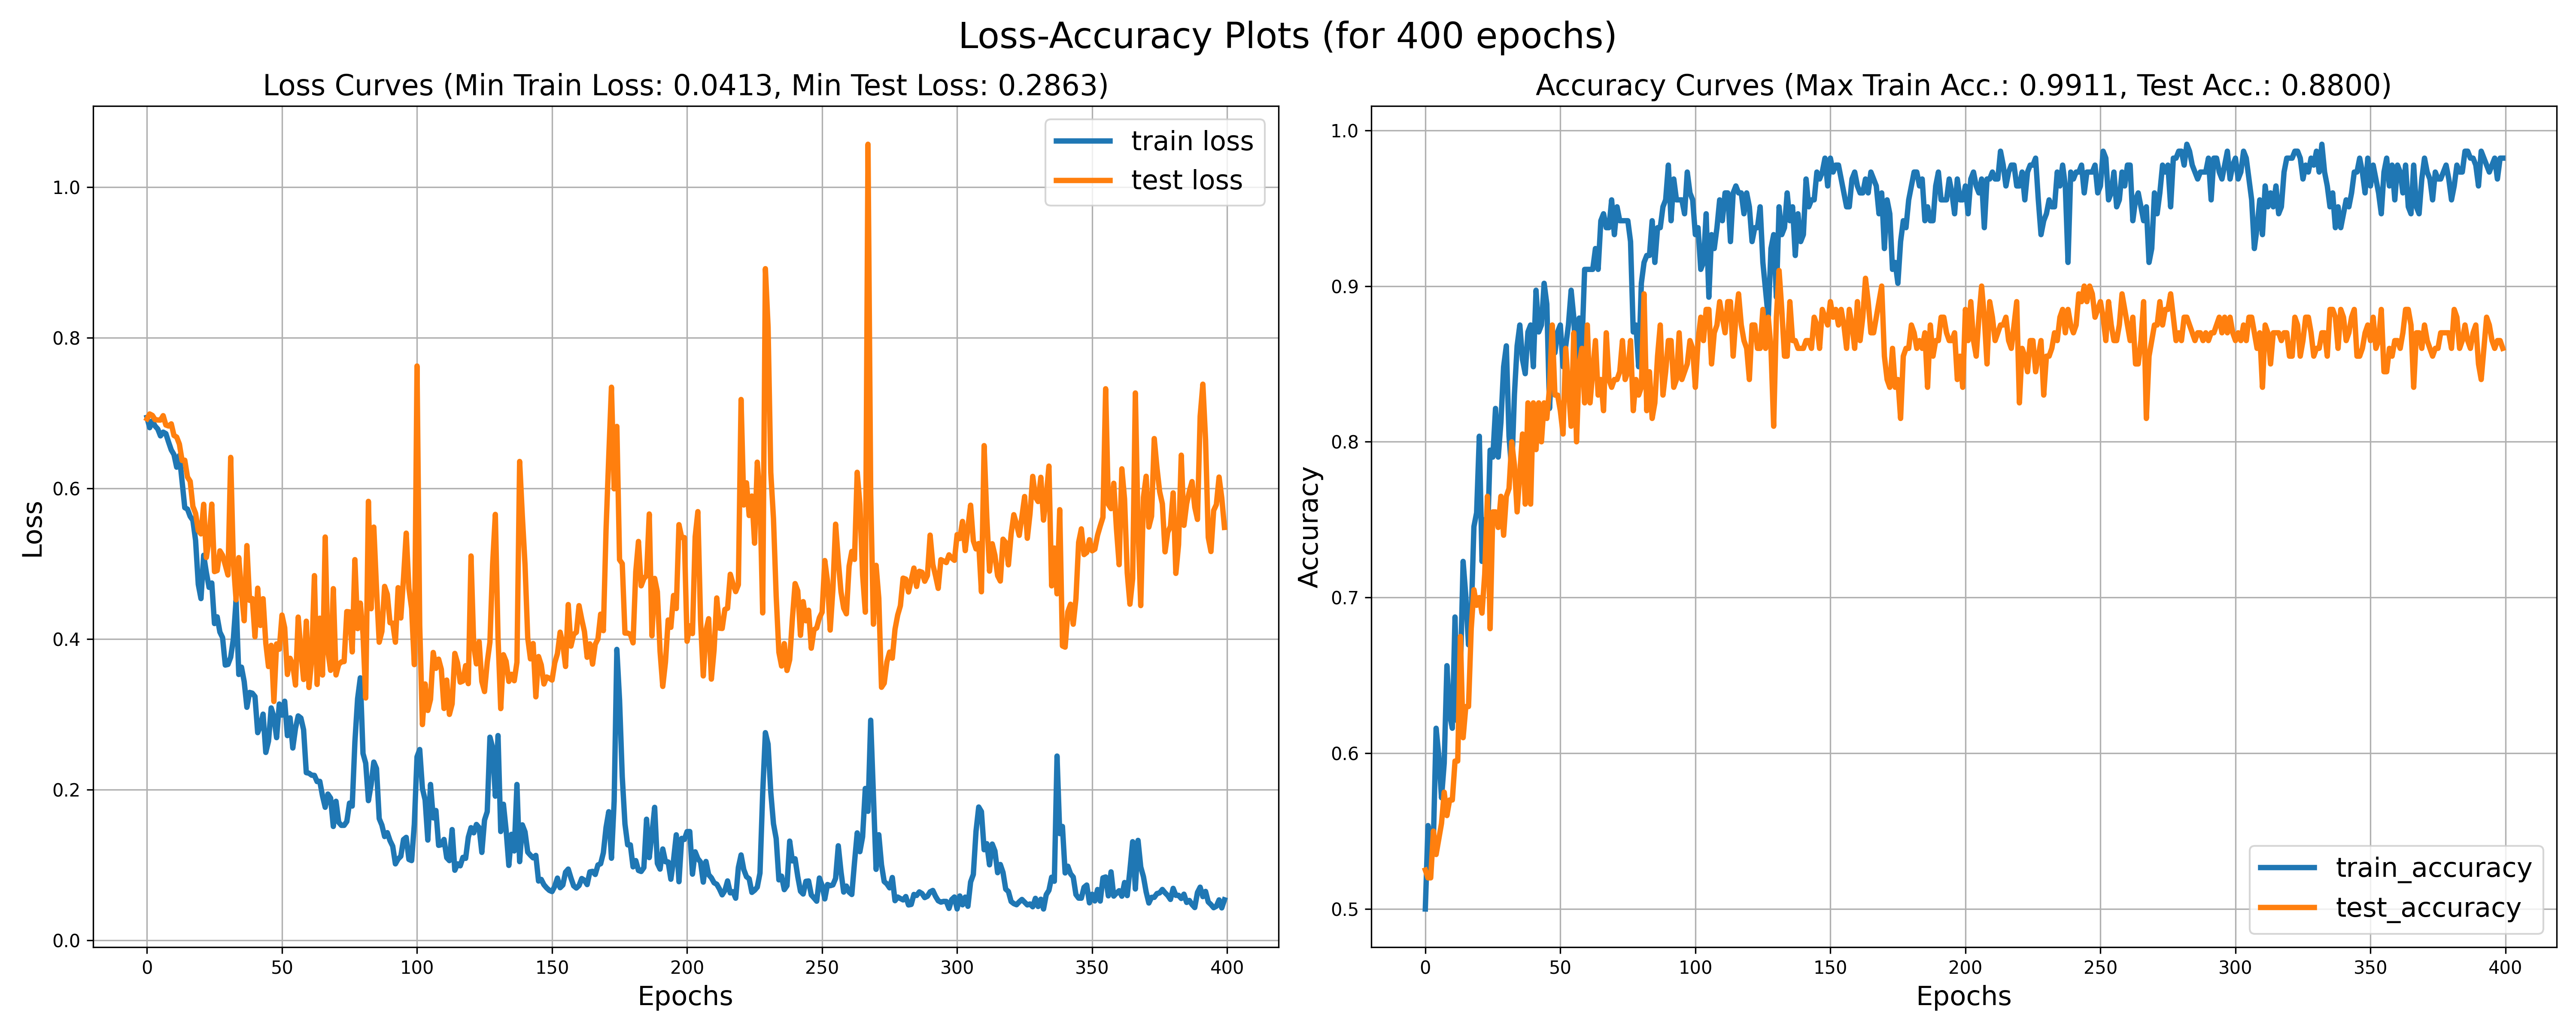
\includegraphics[width=0.9\textwidth]{plots/sinusoid_adam-lr1e-2_more_paramsloss_acc.png}
    \caption{Loss and accuracy for Circle dataset (train, test set with 200 points each)\\ Adam optimizer (lr $=1e-2$ ), 400 epochs, Cost function: CrossEntropyLoss, Xaiver initialization}
    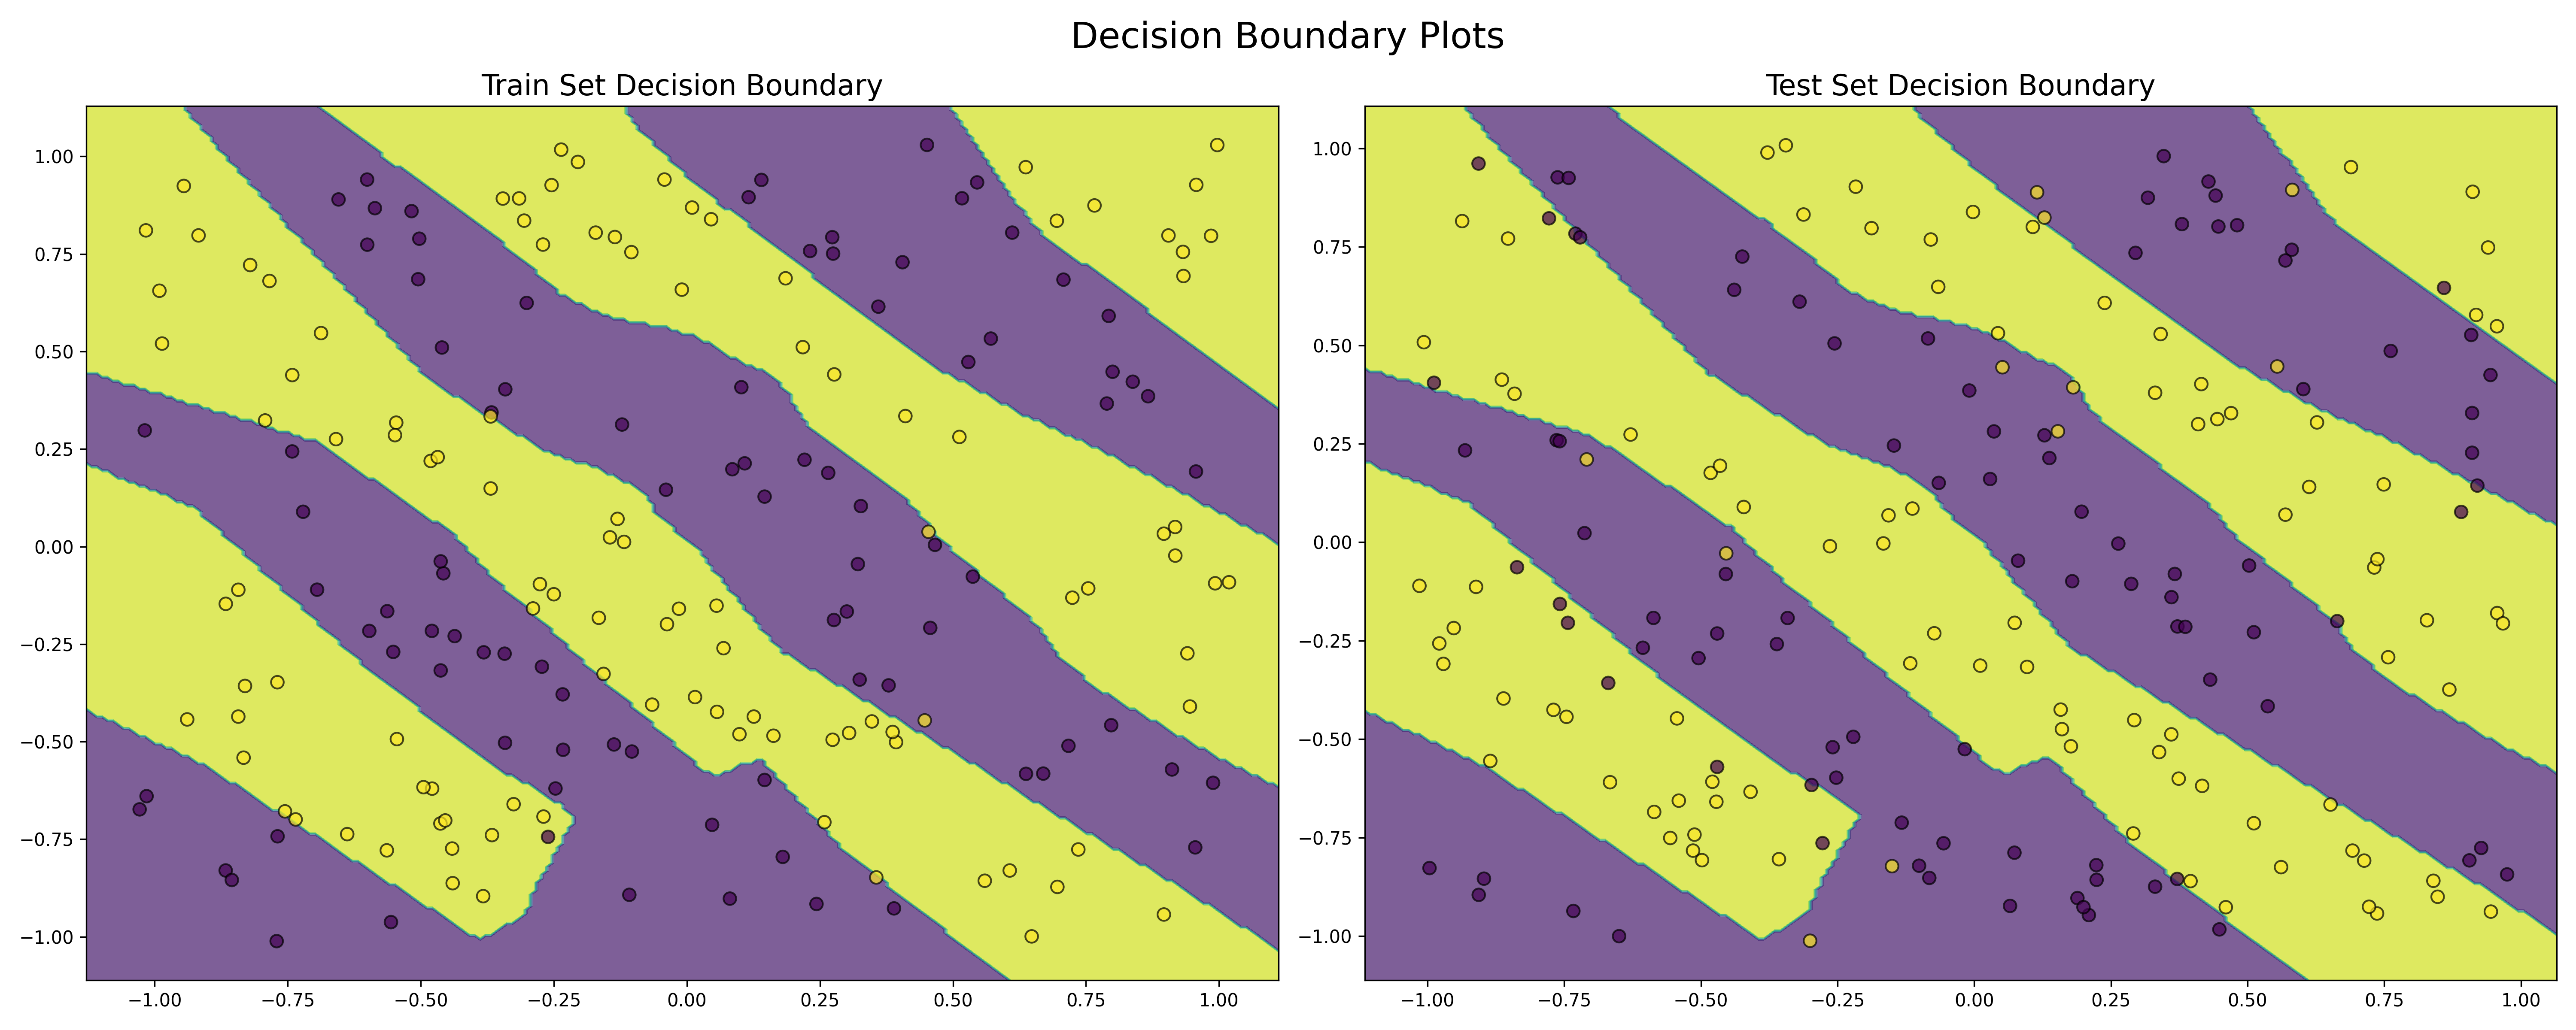
\includegraphics[width=0.8\textwidth]{plots/sinusoid_adam-lr1e-2_more_paramsboundary.png}
    \caption{(L2Loss) Decision boundary for Circle separable dataset (train, test set with 200 points each) 
    Adam optimizer (lr $=1e-2$ )}
\end{figure}

\subsection{MLP with SGD Optimizer of learning rate 0.01 and default parameters (no momentum, no weight decay)}

\begin{figure}[H]
    \centering
    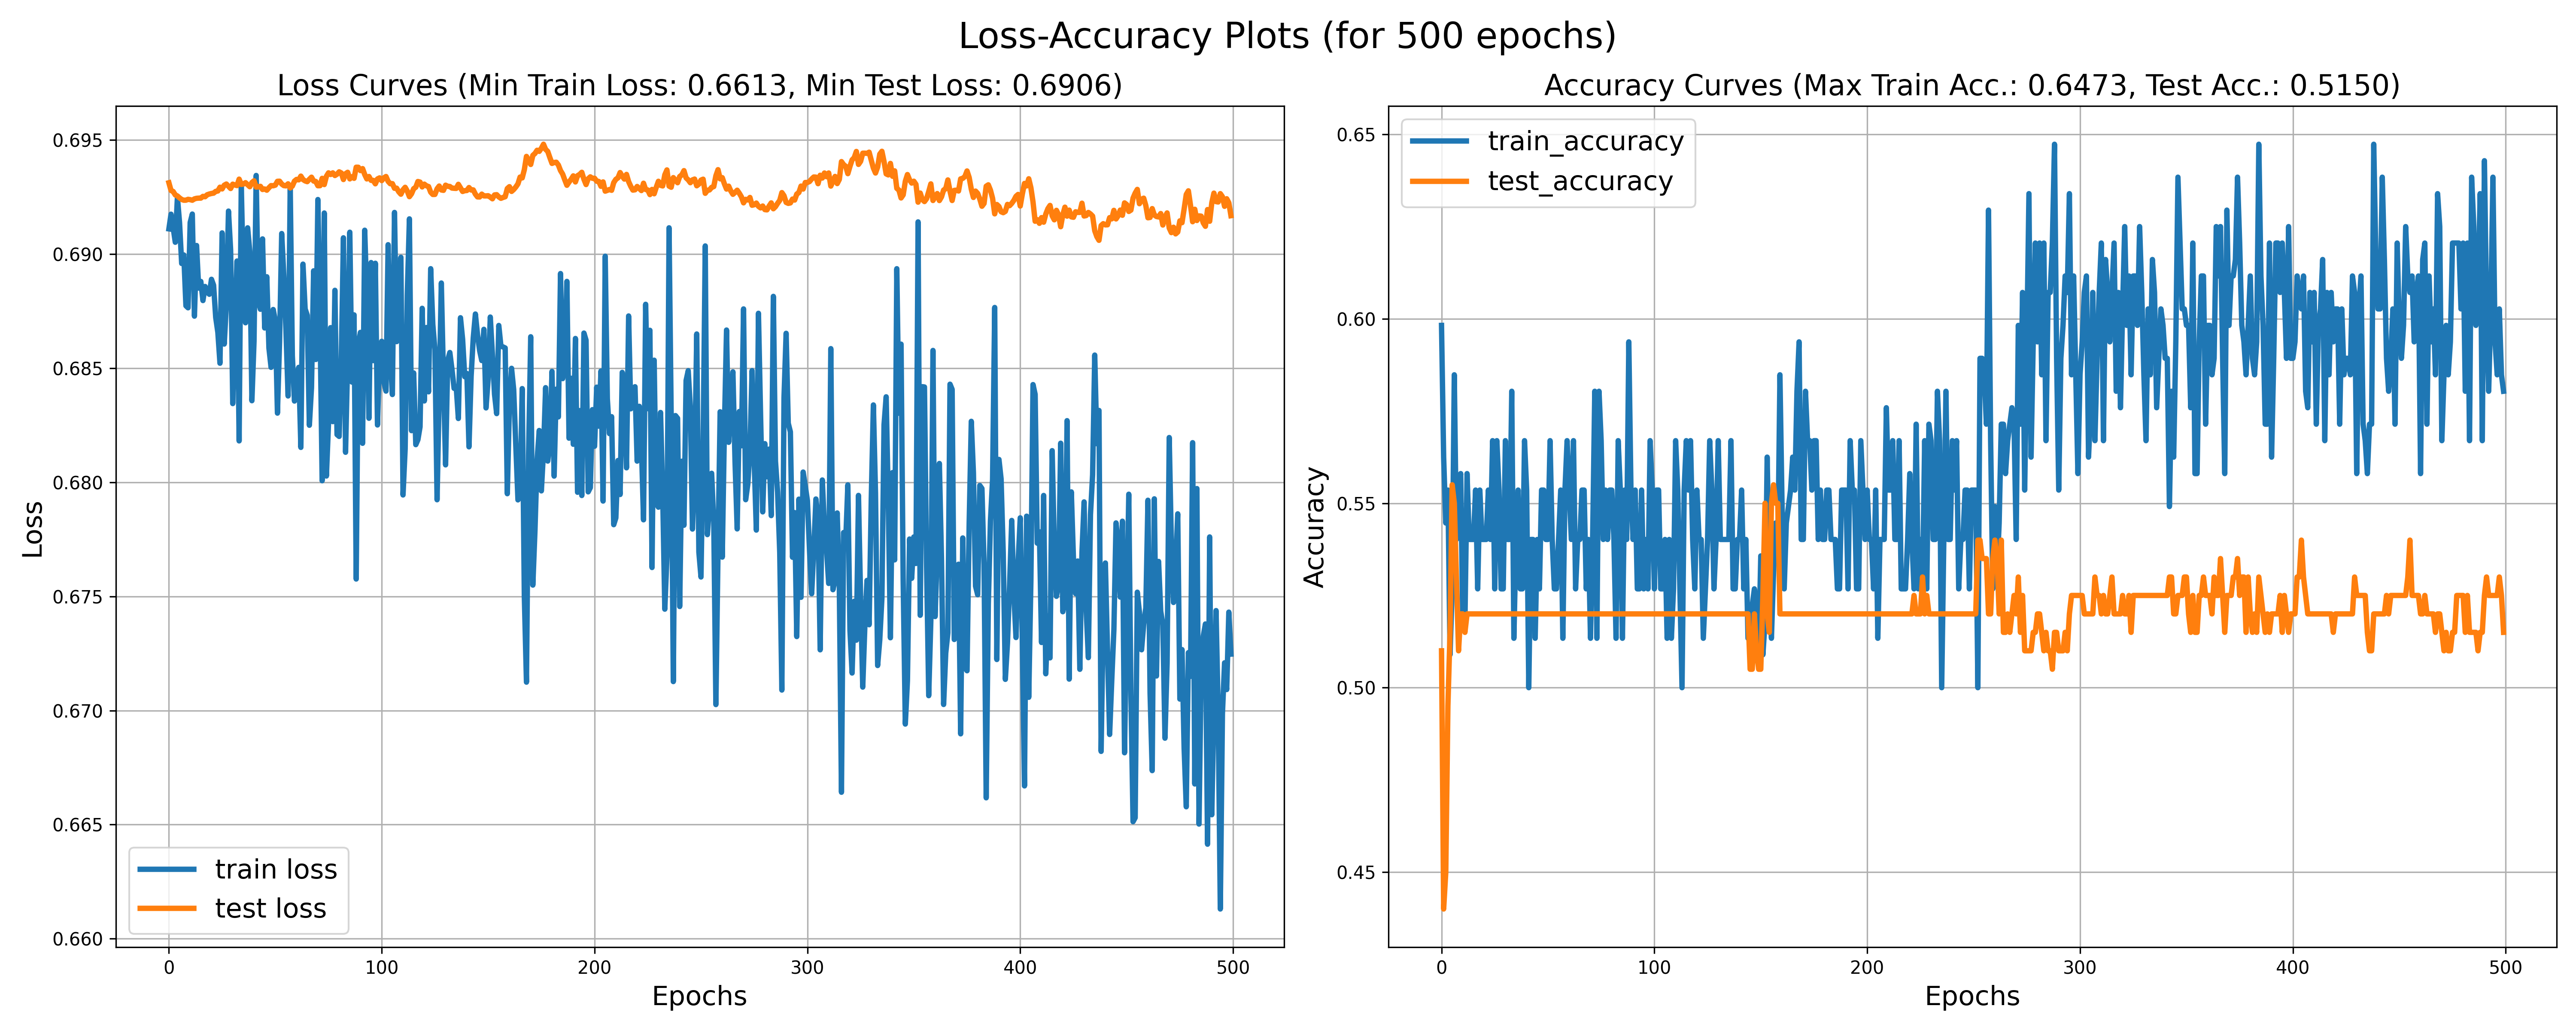
\includegraphics[width=0.9\textwidth]{plots/5_sinusoid_sgd_morelayers_loss_acc.png}
    \caption{Loss and accuracy for Circle dataset (train, test set with 200 points each)\\ SGD optimizer (lr $=1e-2$), 400 epochs, Cost function: CrossEntropyLoss, Xaiver initialization}
    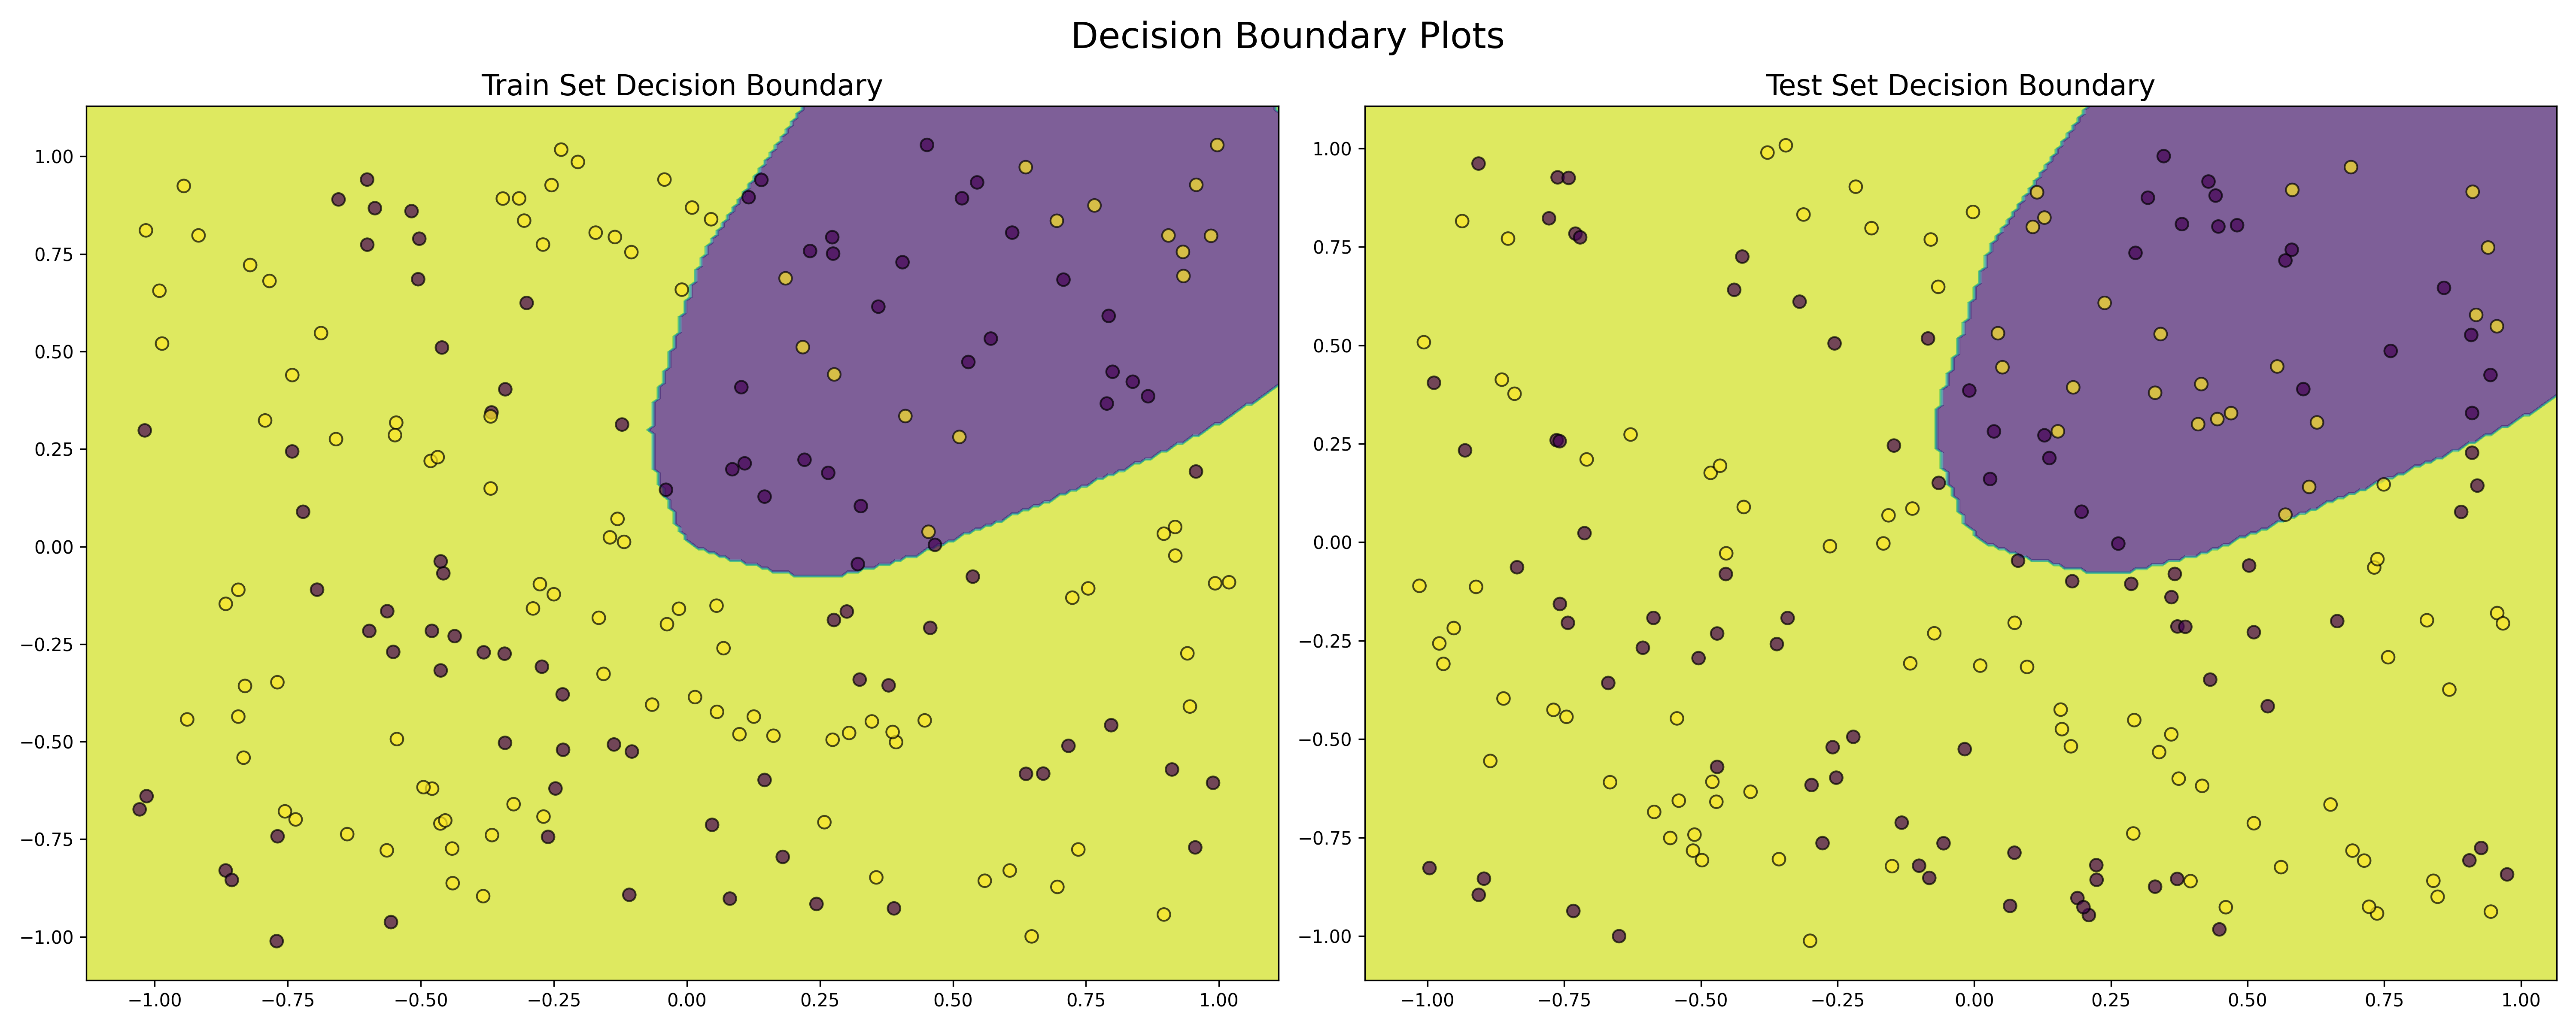
\includegraphics[width=0.8\textwidth]{plots/5_sinusoid_sgd_morelayers_boundary.png}
    \caption{(L2Loss) Decision boundary for Circle separable dataset (train, test set with 200 points each) 
    SGD (lr $=1e-2$ )}
\end{figure}

\subsection{MLP with SGD Optimizer of learning rate 0.01 momentum 0.9, no weight decay}

\begin{figure}[H]
    \centering
    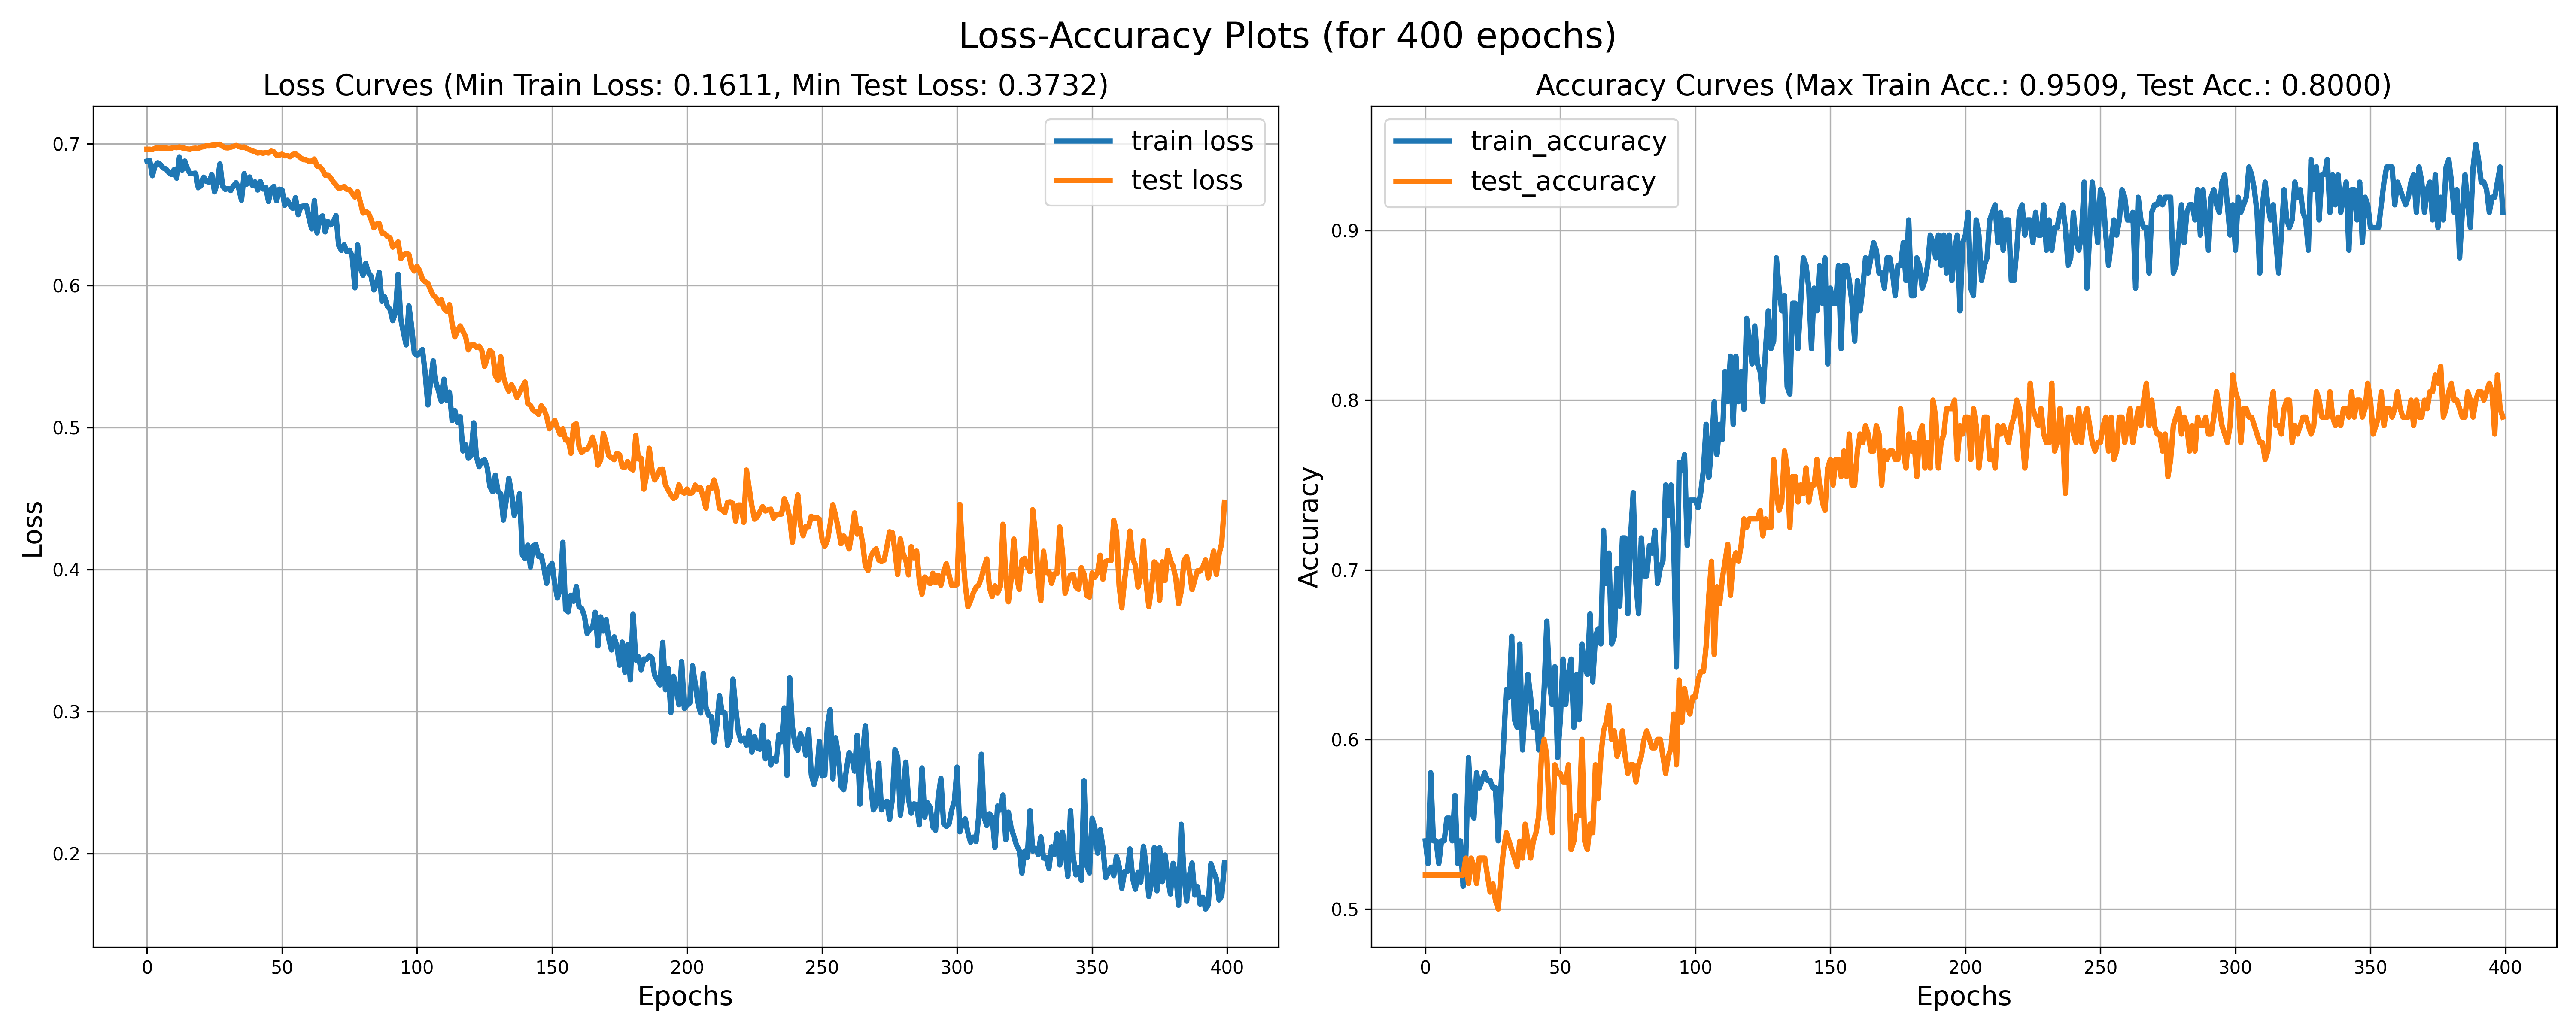
\includegraphics[width=0.9\textwidth]{plots/sinusoid_adam-lr-1e-3_more_layersloss_acc.png}
    \caption{Loss and accuracy for Circle dataset (train, test set with 200 points each)\\ Adam optimizer (lr $=1e-3$ ), 400 epochs, Cost function: CrossEntropyLoss, Xaiver initialization}
    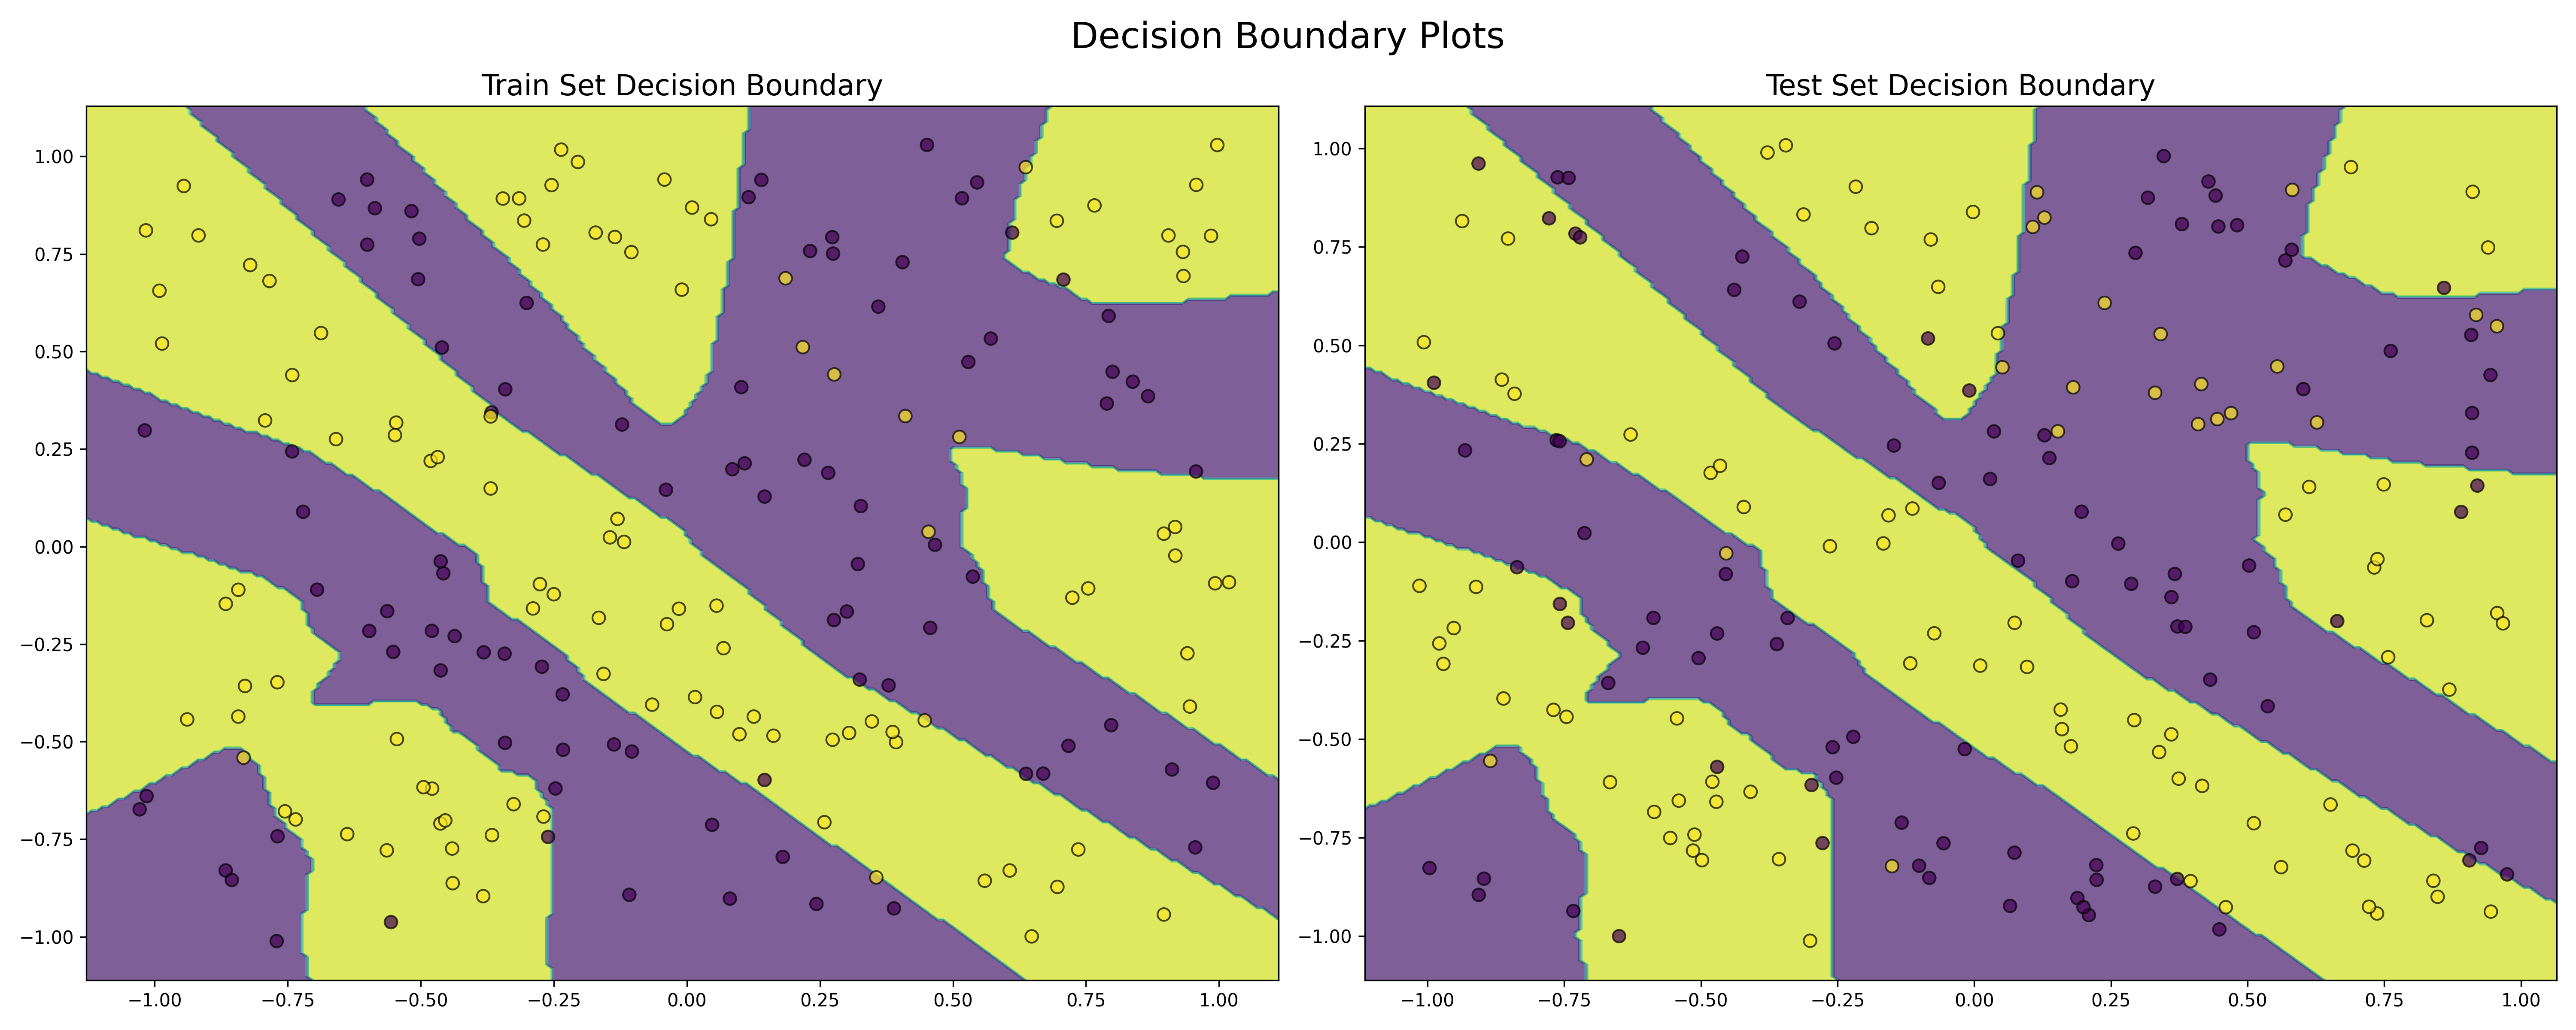
\includegraphics[width=0.8\textwidth]{plots/sinusoid_adam-lr-1e-3_more_layersboundary.png}
    \caption{(L2Loss) Decision boundary for Circle separable dataset (train, test set with 200 points each) 
    Adam optimizer (lr $=1e-3$)}
\end{figure}





\subsection{MLP with Adam Optimizer of learning rate 0.001 and default parameters}

\begin{figure}[H]
    \centering
    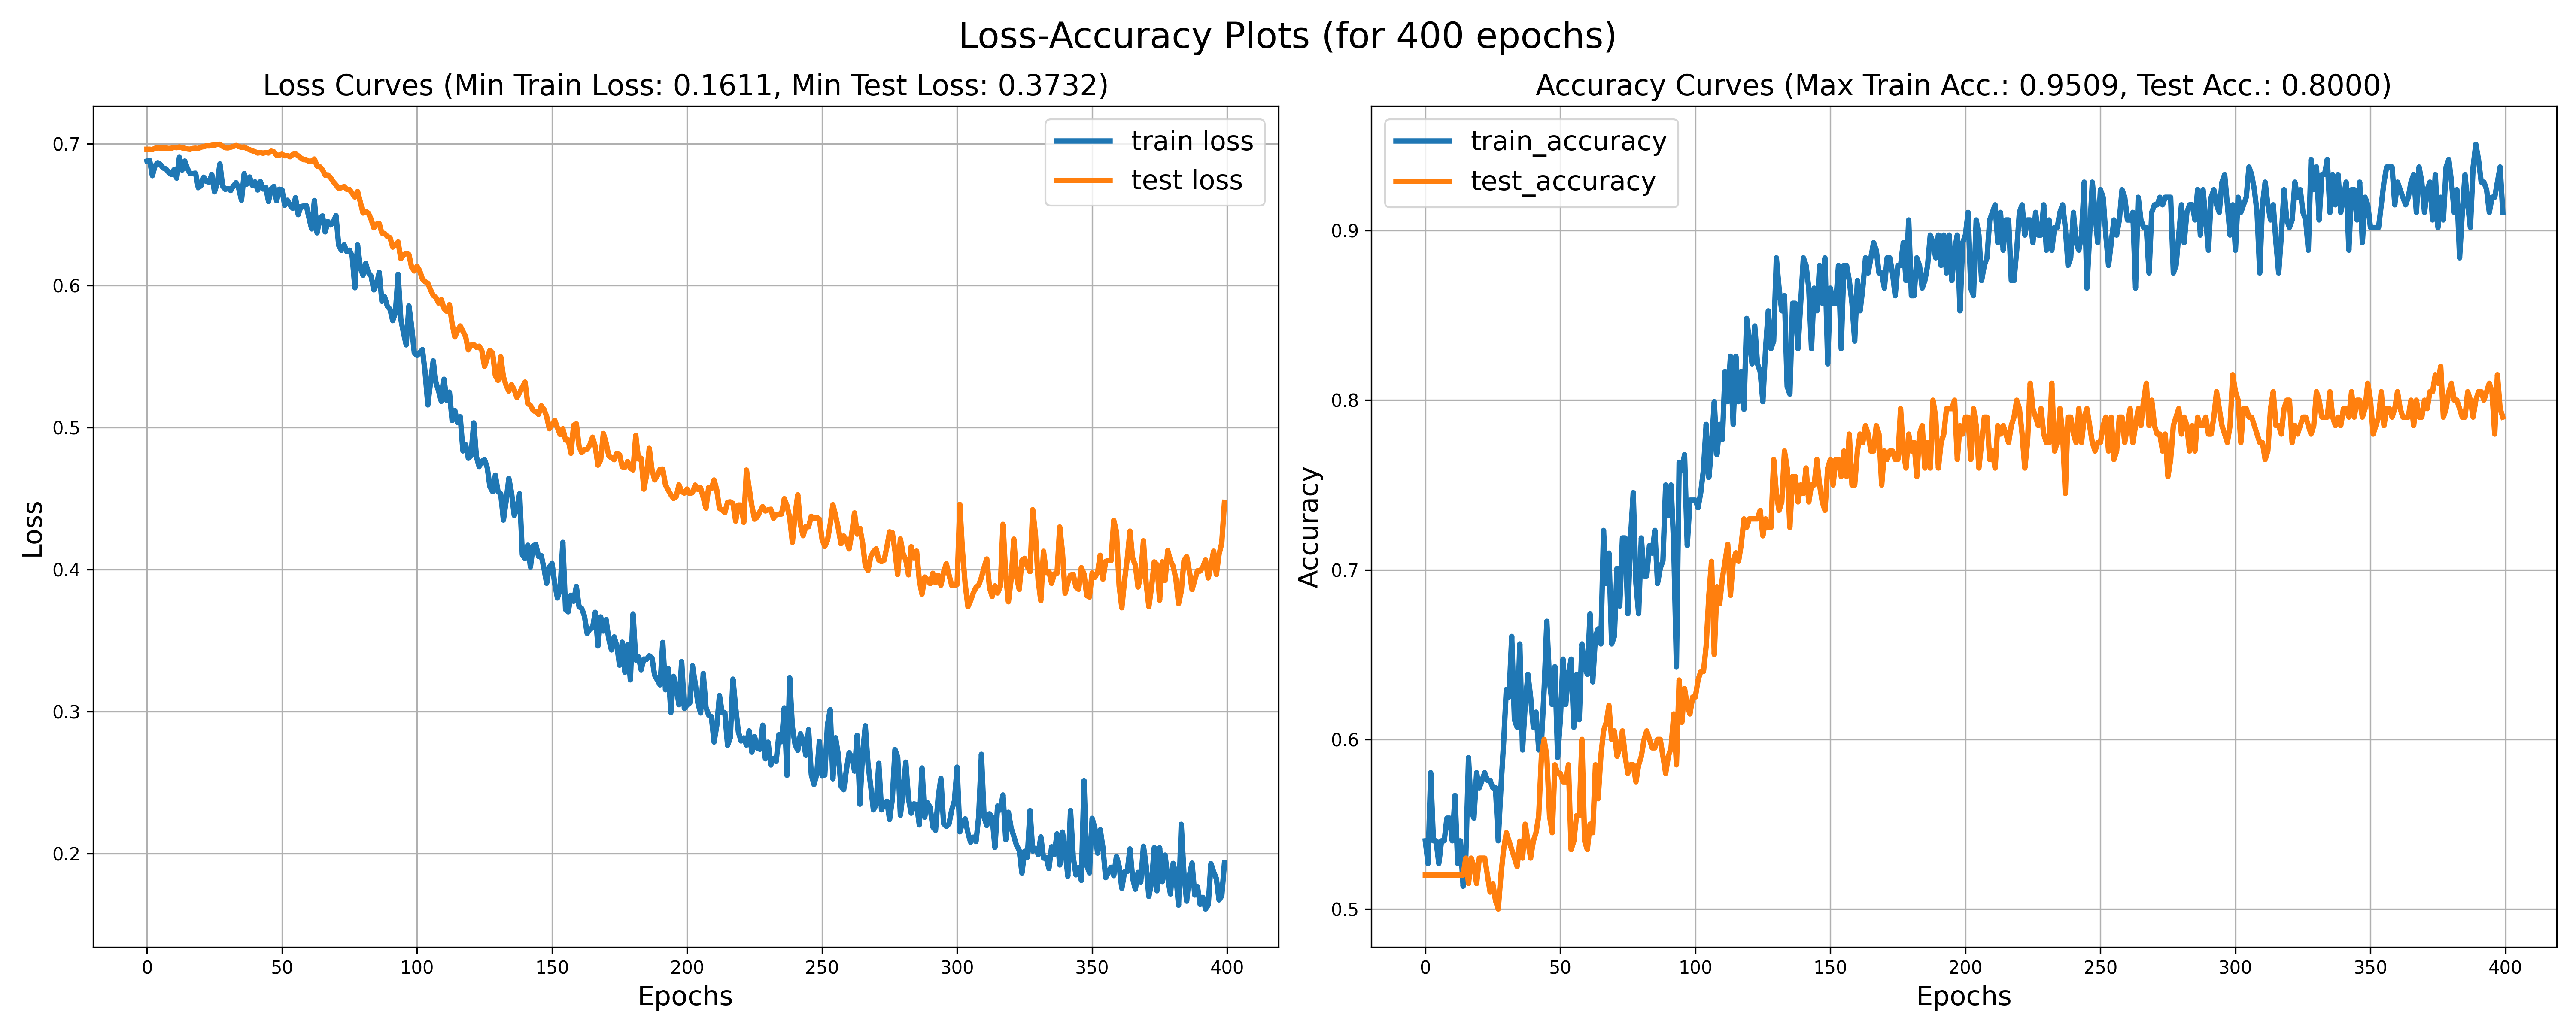
\includegraphics[width=0.9\textwidth]{plots/sinusoid_adam-lr-1e-3_more_layersloss_acc.png}
    \caption{Loss and accuracy for Circle dataset (train, test set with 200 points each)\\ Adam optimizer (lr $=1e-3$ ), 400 epochs, Cost function: CrossEntropyLoss, Xaiver initialization}
    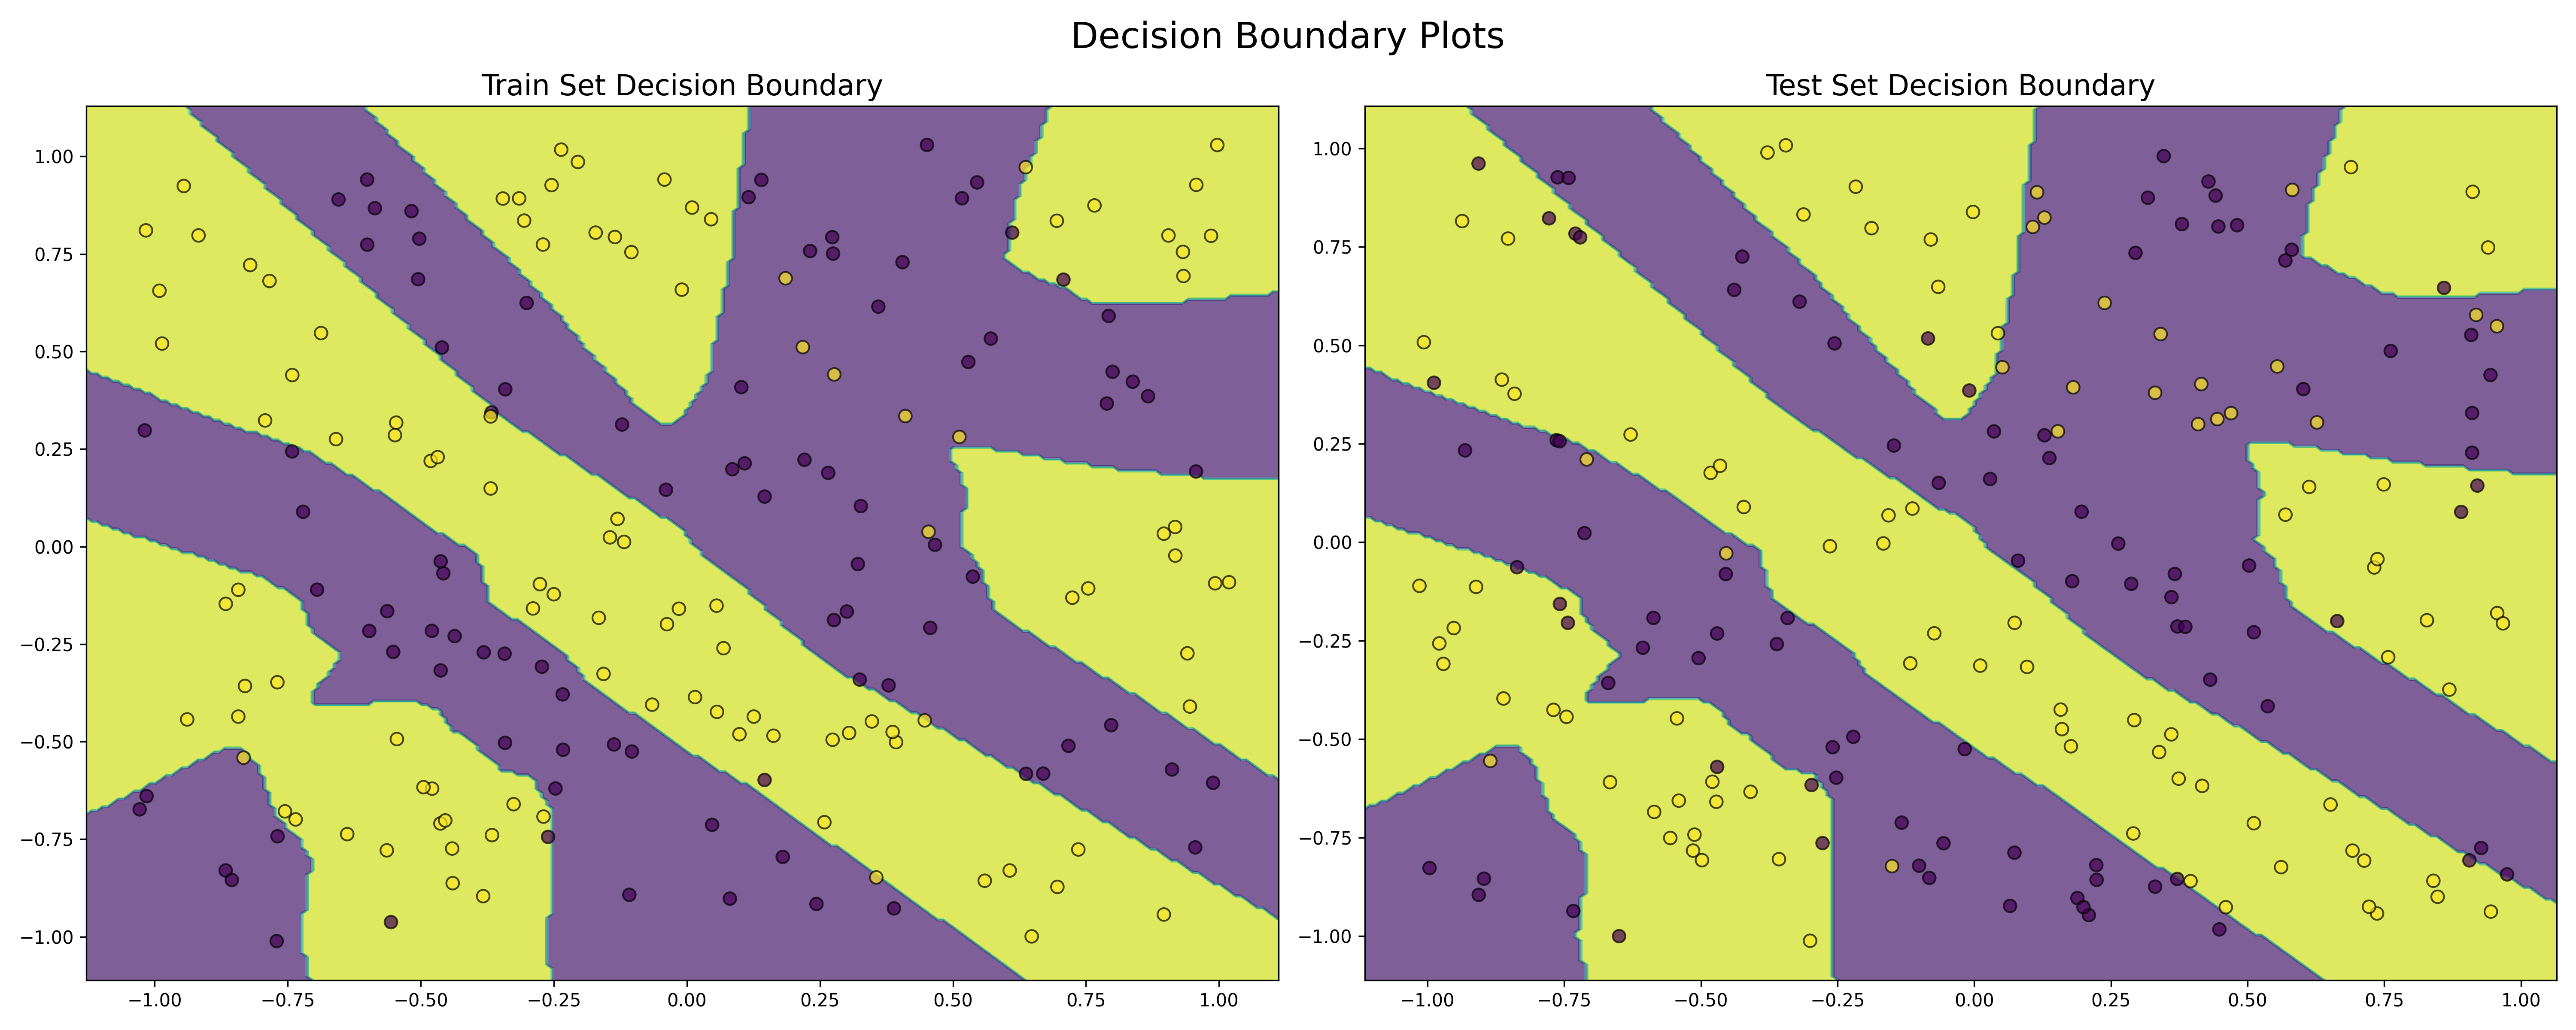
\includegraphics[width=0.8\textwidth]{plots/sinusoid_adam-lr-1e-3_more_layersboundary.png}
    \caption{(L2Loss) Decision boundary for Circle separable dataset (train, test set with 200 points each) 
    Adam optimizer (lr $=1e-3$)}
\end{figure}


% ############################################


\end{solve}
